\label{sec:cnninterrupt}


% Table generated by Excel2LaTeX from sheet 'Sheet3'
\begin{table}[t]
	\centering
	\scriptsize
	\caption{Description for the basic instructions}
% Table generated by Excel2LaTeX from sheet 'Sheet5'
% Table generated by Excel2LaTeX from sheet 'Sheet5'
\begin{tabular}{|p{4em}|p{12em}||p{6em}|p{6em}|}
	\hline
	Type  & Description & Backups & Recovery \bigstrut\\
	\hline
	LOAD  & Load weights/input data/bias from DDR to on chip weight buffer. & -     & Weight / Inputdata \bigstrut\\
	\hline
	CALC\_I & Calculate intermediate results for some output channels from partial  input channels. & Previous final results / Intemediate data  & Weight / Inputdata /  intemediate data \bigstrut\\
	\hline
	CALC\_F & Calculate the results for some output channels from all input channels. & Finial results & Weight / Inputdata \bigstrut\\
	\hline
	SAVE  & Save the results from on-chip data buffer to DDR. & -     & Weight / Inputdata \bigstrut\\
	\hline
	\end{tabular}%
	
	\label{tab:instr}%
  \end{table}%
  

% \begin{figure}[t]
% 	\centering
% 	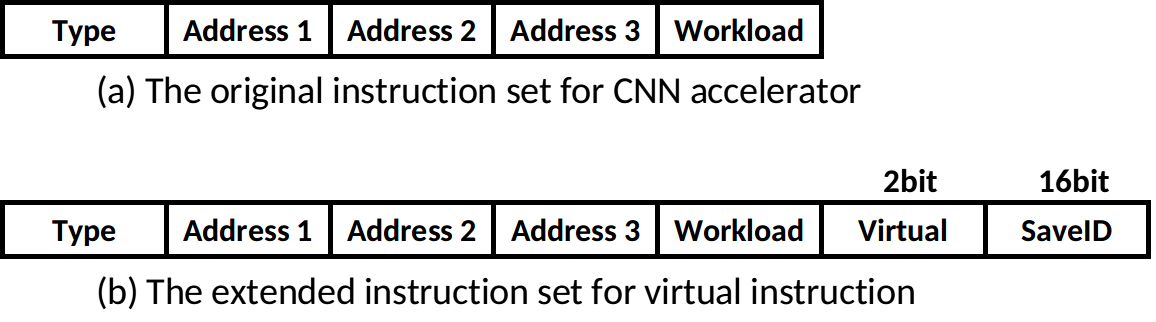
\includegraphics[width=0.9\linewidth]{fig/instructions.png}
% 	\caption{Original and Virtual-Instruction ISA.}
% 	\label{fig:instructions}
% \end{figure}



\subsection{ Instruction Driven Accelerator }
\label{sec:instrAcc}
There are three categories of instruction in the instruction-driven accelerator: LOAD, CALC (CALC\_I / CALC\_F), and SAVE  ~\cite{guo2017angel,qiu2016going,yu2018instruction}. The instruction description of each kind of instruction is listed in \Cref{tab:instr}. 

Each CALC  instruction,  including CALC\_I and CALC\_F, processes the convolution according to the hardware parallelism with $Para_{height}$ lines from $ Para_{in} $ input channels to $ Para_{out}$ output channels. $Para_{height}$, $ Para_{in} $, and $ Para_{out} $ are the parallelism along the height, input channel and output channel dimensions, which is determined by the hardware and original ISA. The convolution of the last $ Para_{in} $ input channels is CALC\_F, and the convolutions for the former input channels are CALC\_I, as illustrated in \Cref{fig:singlesave}(a). The CALC\_F and the CALC\_I instructions for the same output channels, as well as the LOAD instructions for corresponding input feature-maps and weights, are considered as a \textbf{CalcBlob}.


\begin{figure}[t]
    \centering
	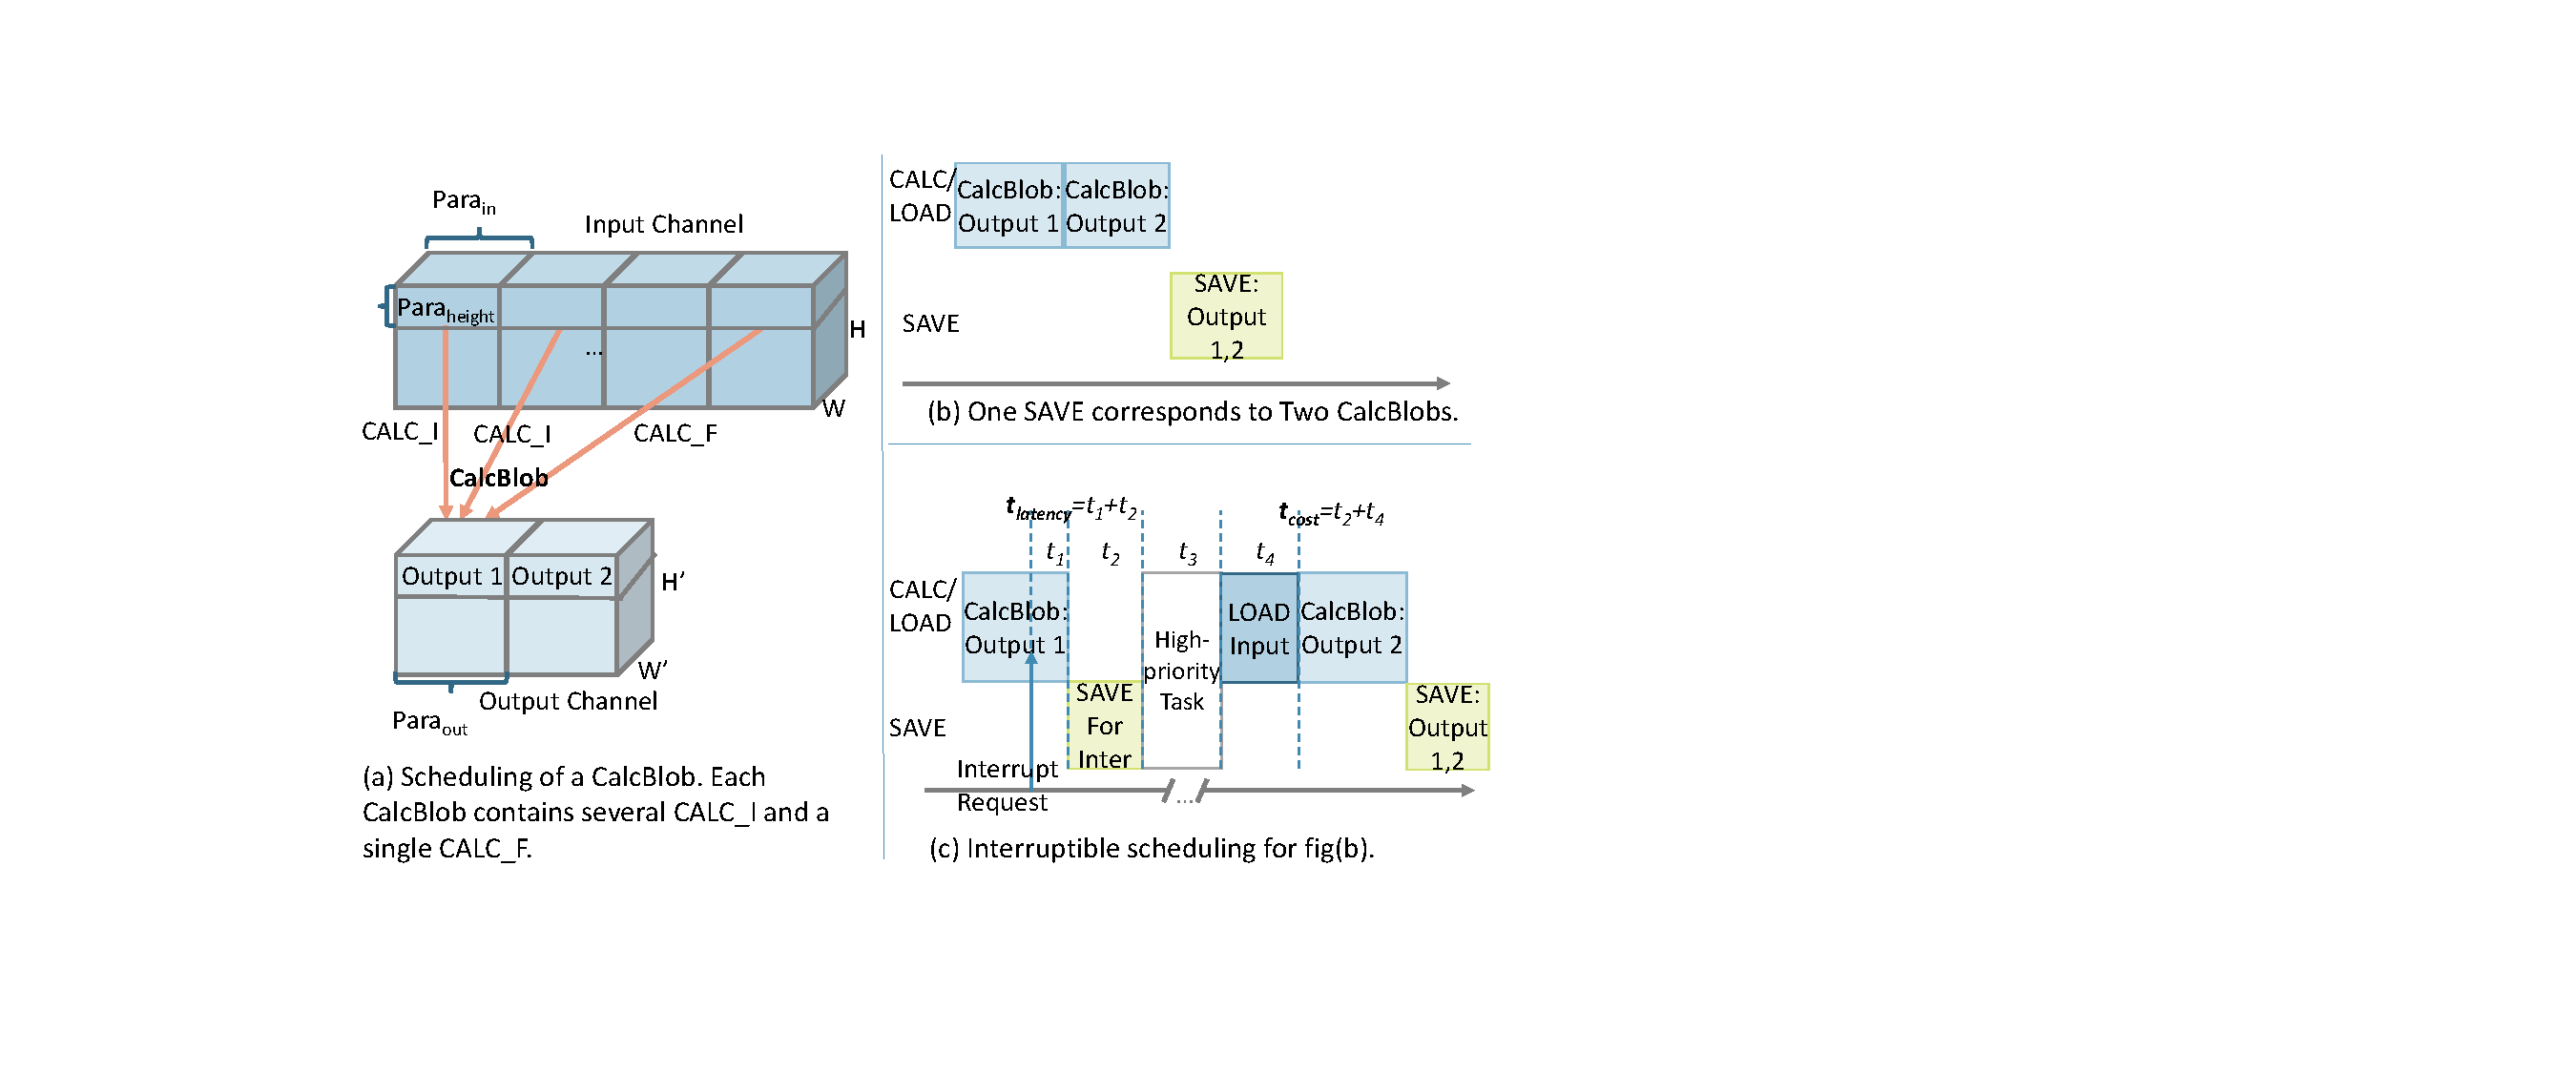
\includegraphics[width=1.04\linewidth]{fig/singlesave.pdf} 	
    \caption{
		Scheduling Illustration
    }
	\label{fig:singlesave}
\end{figure}

\subsection{How To Interrupt: Virtual Instruction}
\label{sec:howinter}

There are four stages to handle interrupt. For the instruction flow illustrated in \Cref{fig:singlesave}(b), the interrupt stages are shown in \Cref{fig:singlesave}(c), including: (1) Time for finishing the current operation, $t1$. (2) Time to backup, $t2$. (3) Time for the high-priority task, $t3$. (4) Time to restore the low-priority task ,$t4$. The the latency to respond the interrupt is $t_{latency} = t_1+t_2$. The extra cost for interrupt is $t_{cost}=t_2+t_4$. 
There are different methods to implement interrupt in CNN accelerators.

\textbf{CPU-Like.}
When an interrupt request occurs in CPU, CPU backs up all the on-chip registers to DDR. However, there are only tens of registers in CPU, and the volume of the backed-up data is less than 1 KB  ~\cite{furber2000arm}. In CNN accelerators, there are several $MB$ of on-chip caches  ~\cite{qiu2016going, guo2017angel} for input feature-maps and weights. 
% If all on-chip caches are backed-up/recovered, the cost of data transfer in the accelerator is much higher than that of CPU. 
Thus, the extra data transfer increases both the interrupt response latency($t_{latency}$) and the additional cost ($t_{cost}$).

\textbf{Layer-by-layer.}
Most accelerators run the CNN layer by layer  ~\cite{qiu2016going,guo2017angel}. 
There is no extra data transfer for the accelerator to switch between different tasks after each layer, thus, $t_{cost}=0$. 
However, the position of the interrupt request is irregular and unpredictable. When an interrupt occurs inside a CNN layer, the CNN accelerator needs to finish the whole layer before switching, which leads to the high response latency($t_{latency}$).

% The latency to respond the interrupt and the performance degradation of the CPU-like interrupt and Layer-by-layer method will be evaluated in \Cref{sec:experiments}.

We propose the \textbf{virtual-instruction-based} method (VI method) to enable low-latency interrupt. 
% Different from the CPU-like interrupt, which backup/recovery all the on-chip caches, only the on-chip cache which is still needed in future execution will be backed-up and restored. So that the amount of data transfer is much lower than that of CPU-like interrupt.
To reduce the interrupt response latency, our virtual-instruction-based method is interruptible inside each layer. We add some virtual instructions to the original instruction sequence to enable the interrupt.
The virtual instructions, which contain the backup and recovery instructions, are responsible for backing up and restoring on-chip caches. 

% \textbf{Virtual SAVE} instructions back up the intermediate results from partial input channels or the final output results. There is no need to back up the input feature-maps and weights, because these inputs are already stored in DDR. 

% \textbf{Virtual LOAD} instructions restore the input feature-maps from DDR to on-chip caches, because input featuremaps are loaded by one CalcBlob, and shared across subsequent CalcBlobs.
% , and thus the subsequent CalcBlobs do not read the input feature-maps. 
% Virtual LOAD instructions also need to restore the intermediate results from partial input channels backed up by the virtual SAVE instructions.


\subsection{ Where To Interrupt: After SAVE/CALC\_F }
\label{sec:whereinter}
% The virtual-instruction-based method has two potential factors that may lead to system performance degradation: 1) The extra data transfer to backup/restore running status takes up additional bandwidth resources. 2) The instruction fetching for the virtual instructions also uses bandwidth resources.
%  Even they are skipped and discarded.
% To address the above problems of virtual-instruction-based method, 
We analyze the interrupt cost and select the positions of adding the virtual instructions.
The backup/recovery data for different interrupt positions at each kind of instruction are listed in the Backup/Recovery columns of \Cref{tab:instr}.

When an interruption occurs at \textbf{LOAD}, the newly loaded data are immediately flushed when running the high-level CNN, leading to bandwidth waste.

Compared with CALC\_I, when an interrupt occurs at \textbf{CALC\_F}, there are no intermediate results. 
Although it is necessary to back up the unsaved final results which are generated by previous CALC\_F, these results will be stored in DDR through the subsequent original SAVE instruction.
If the accelerator can record the interrupt status, we can modify the address and workload when executing subsequent original not-virtual SAVE instruction.
Thus, we can avoid the repetitive transmission of the final output results.

The overhead of interrupt after \textbf{SAVE} is only to transfer input data from DDR to the on-chip caches. 

In order to minimize the cost of interrupt, we make the CNN interruptible after the SAVE or CALC\_F. This method only introduces extra data transfer to recovery input data without any extra backup data. Thus, $t_{cost} = t_4$, in our virtual-instruction-based interrupt.

% \begin{figure*}[t]
% 	\centering
% 	\subfloat[ $t_1$ for Layer-By-Layer method. ]{ \label{fig:t1all}
% 		\begin{minipage}[t]{0.45\linewidth}
% 			\centering
% 	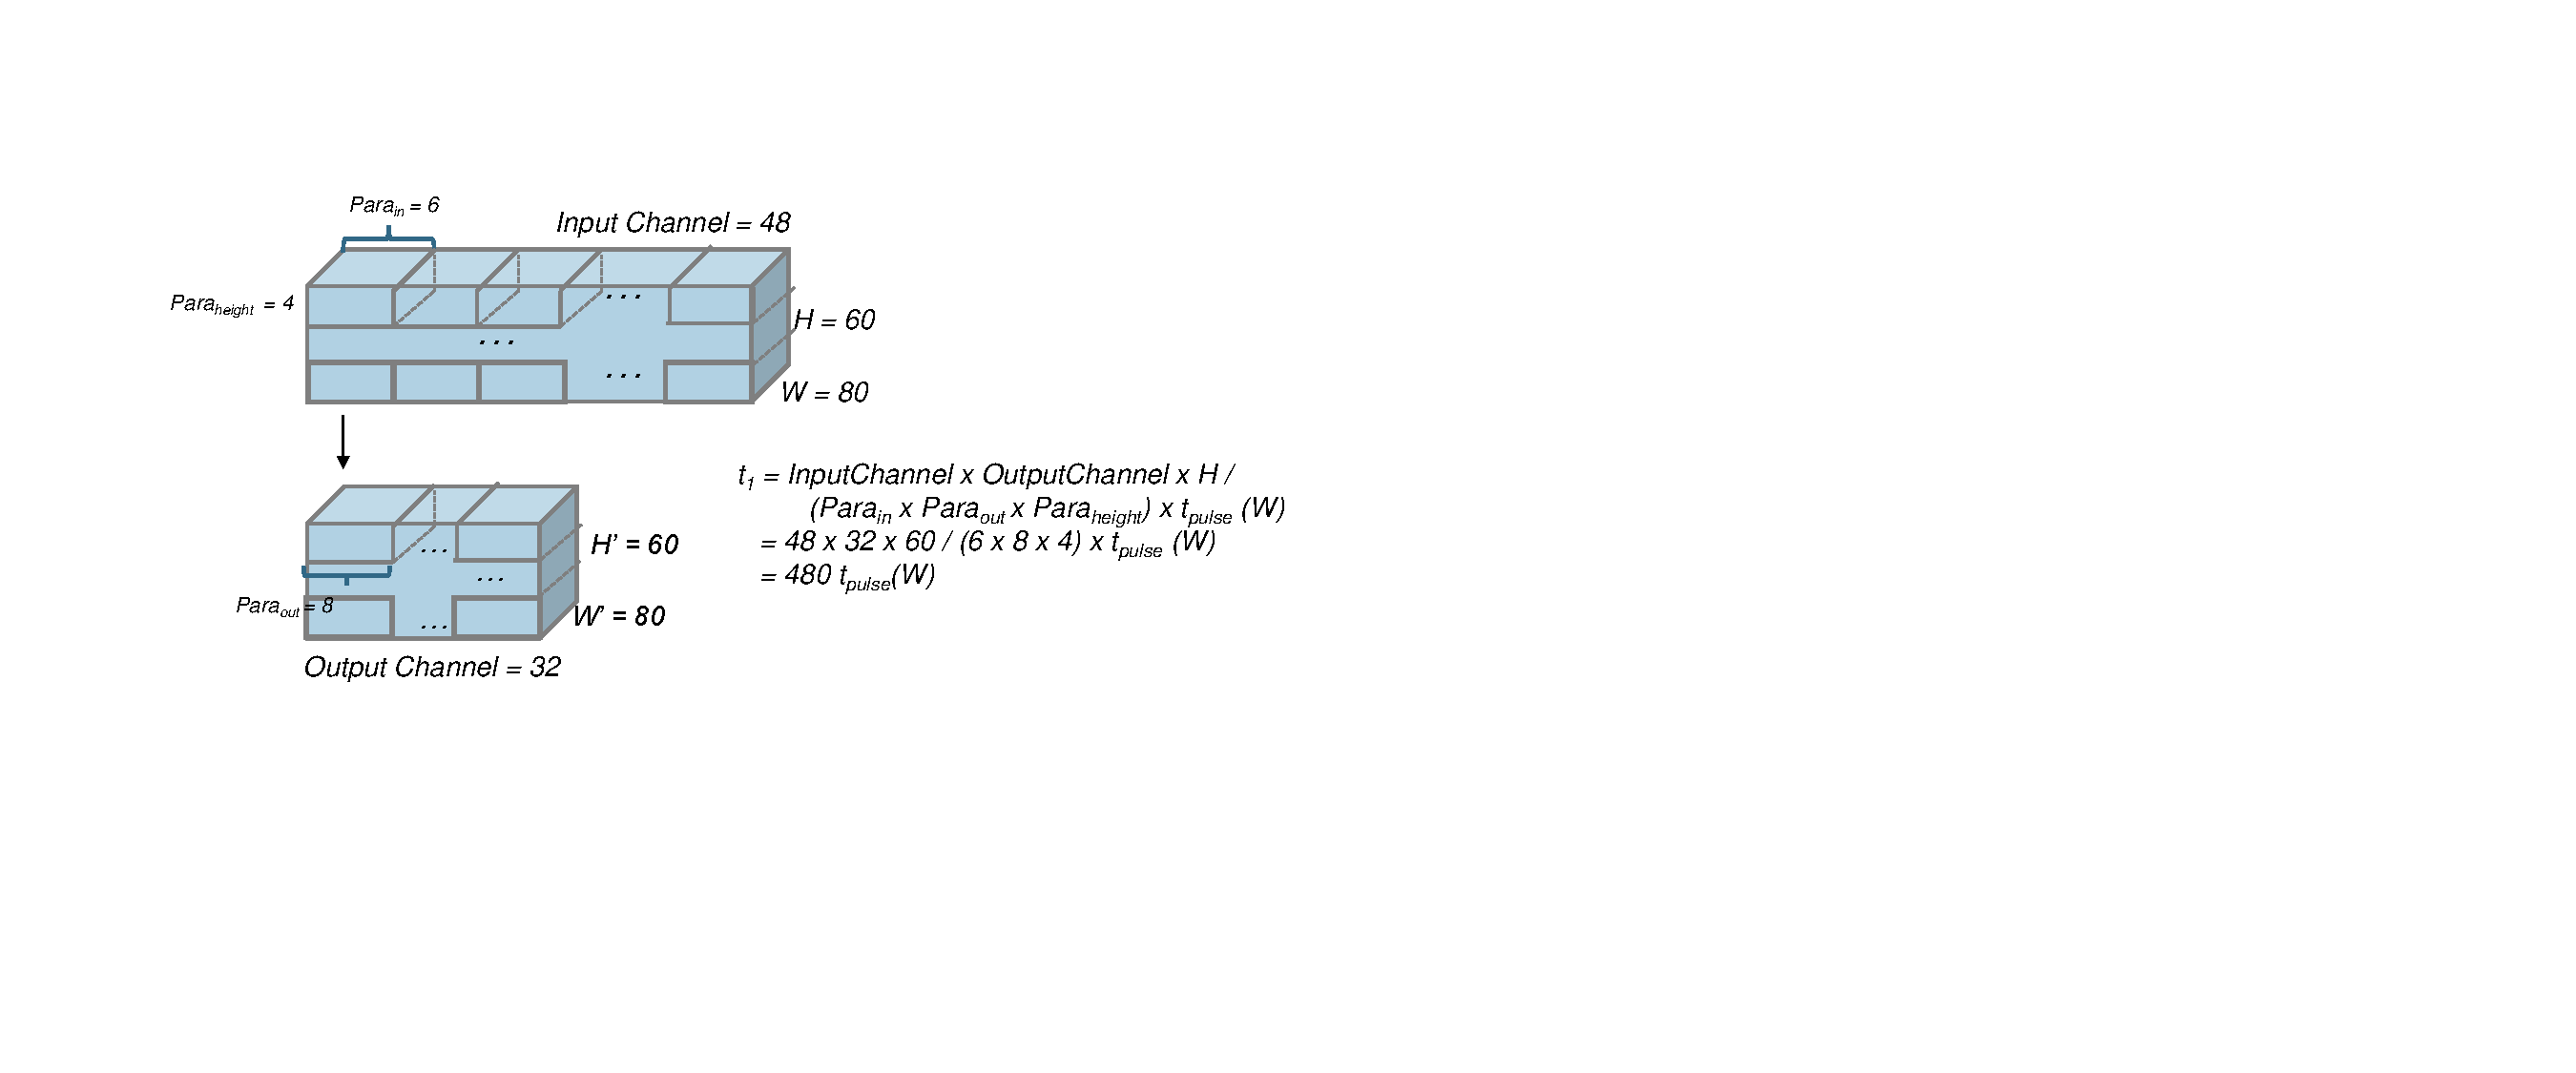
\includegraphics[width=0.99\linewidth]{fig/t1all.pdf}
% 		\end{minipage}%
% 	}
% 	\subfloat[ $t_1$ for Virtual-Instruction method. ]{ \label{fig:t1after}
% 		\begin{minipage}[t]{0.45\linewidth}
% 			\centering
% 	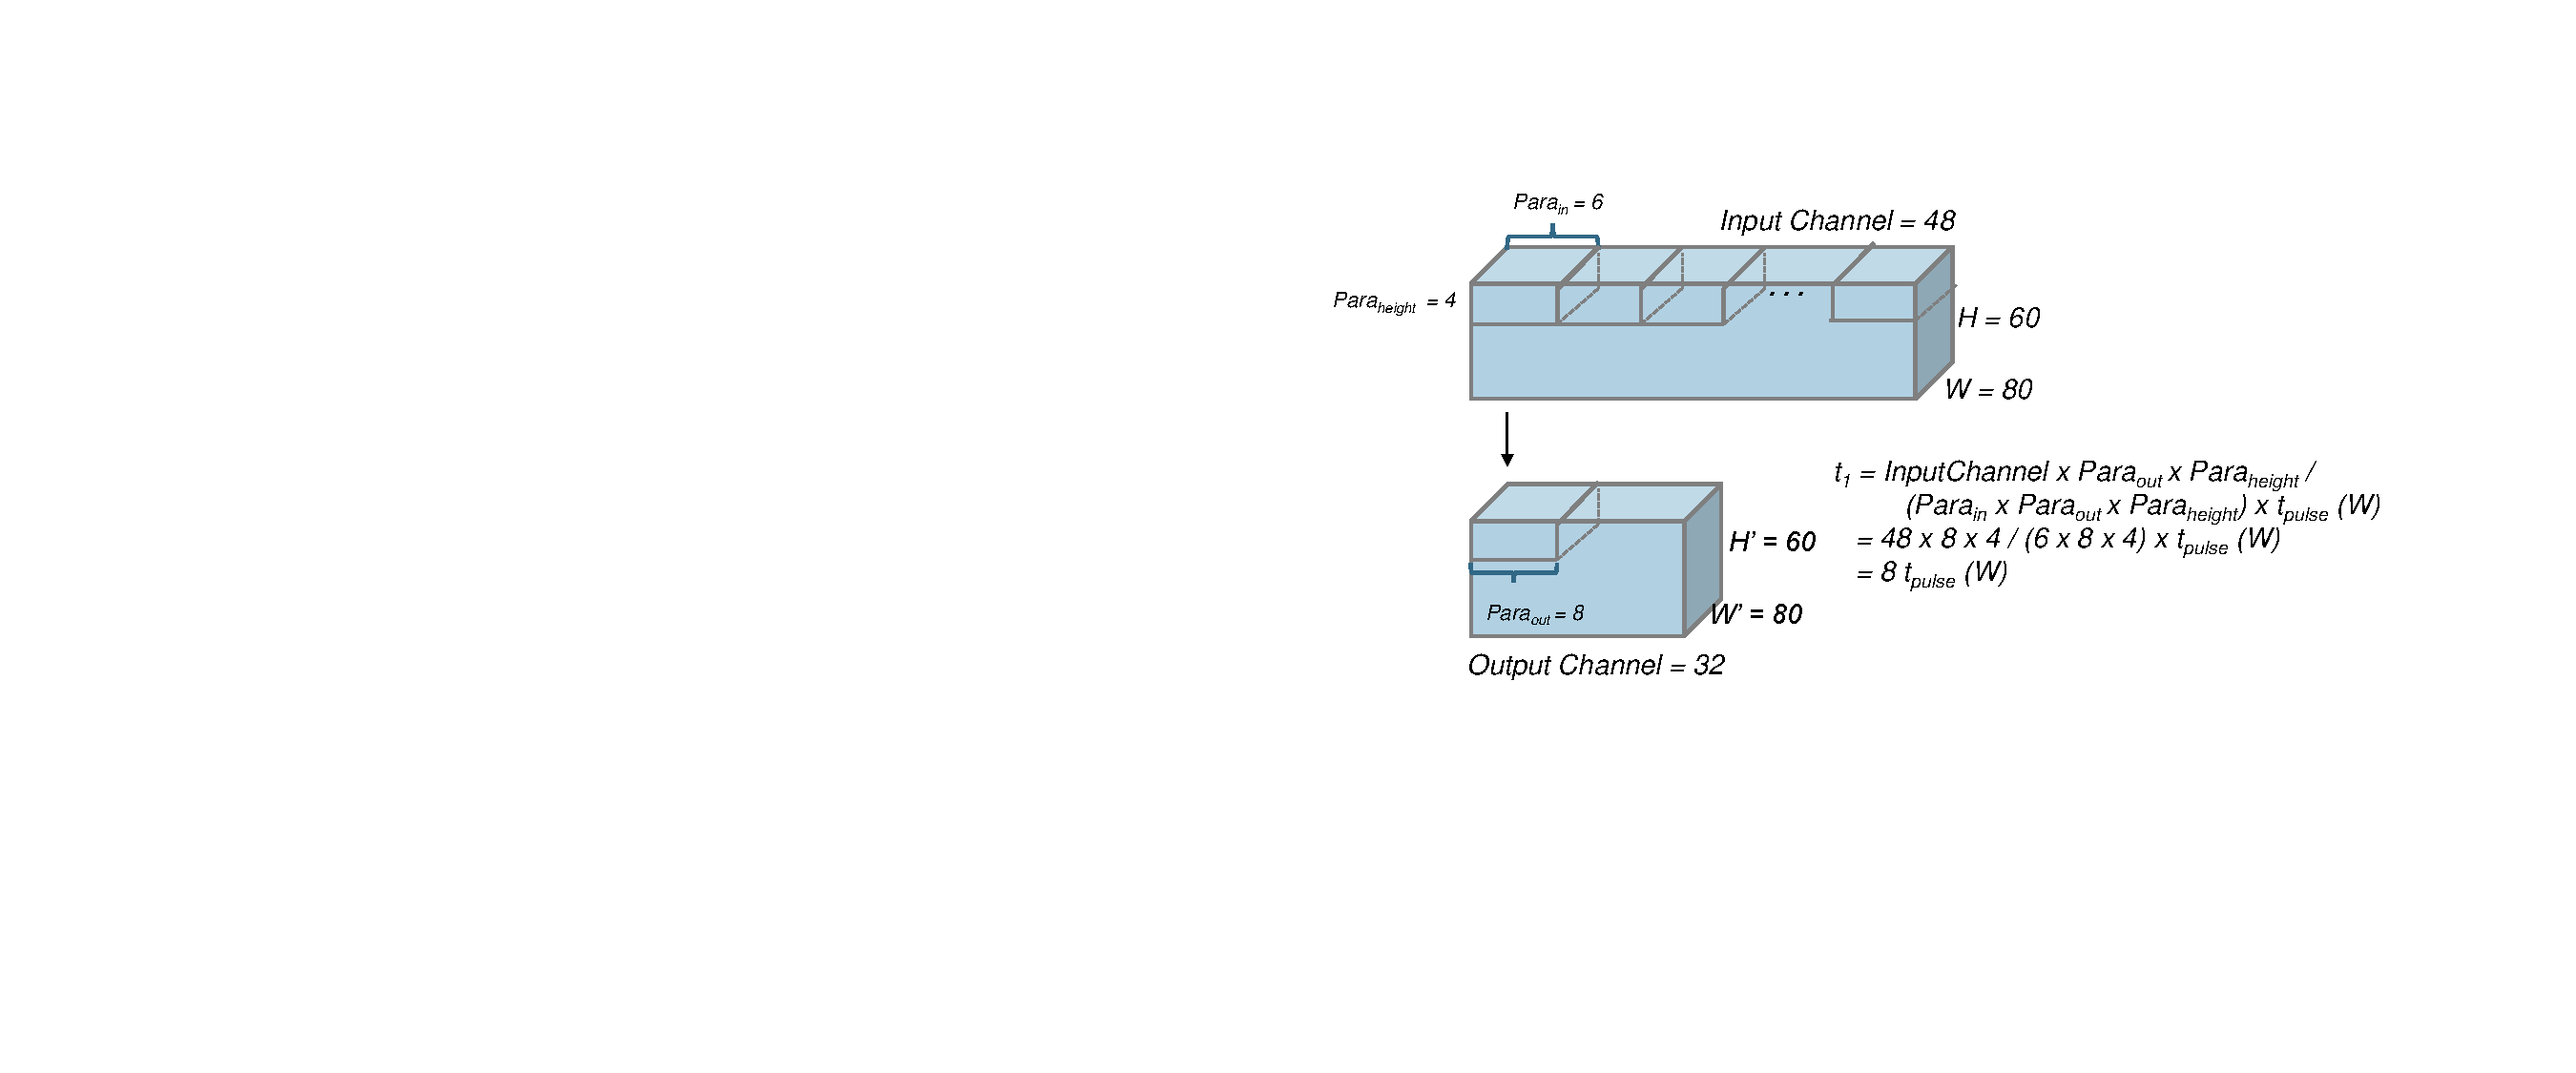
\includegraphics[width=0.99\linewidth]{fig/t1after.pdf}
% 		\end{minipage}%
% 	}
% 	\label{fig:t1example}
% 	\caption{ Waiting time for finishing the current operation ($t_1$) in an example convolution layer. Compared with the Layer-By-Layer method, the waiting time of our Virtual-Instruction method is reduced to $1.6\%$ in this example. The reduction in latency is related to the height ($H$) of the input featuremaps.  }
% \end{figure*}

Compared with Layer-by-layer interrupt, our method, which is interruptible after CALC\_F and SAVE, significantly reduces $t_{latency}$.
In the worst case, the interrupt request occurs at the beginning of the layer. In this case, the accelerator will wait until finishing the whole layer. The wait time is $t_{1\_layer}$:

\begin{equation*}
	t_{1\_layer} = \frac{ Ch_{in} \times Ch_{out} \times H }{ (Para_{in} \times Para_{out} \times Para_{height}) } \times t_{instr}(W)
\end{equation*}

Where $t_{instr}(W)$ is calculation time of a single CALC. The $W$ of the input featuremaps is larger, the time of a single CALC is longer.

The worst wait of our VI method is $t_{1\_VI}$:

\begin{equation*}
	t_{1\_VI} = \frac{ Ch_{in} \times Para_{out} \times Para_{height} }{ (Para_{in} \times Para_{out} \times Para_{height}) }  \times t_{instr}(W)
\end{equation*}

Compared with the Layer-By-Layer method, the worst latency of our method is reduced to $R_l$.

\begin{equation*}
	R_l = \frac{ t_{1\_VI} }{ t_{1\_layer} }  = \frac{ Para_{out} \times Para_{height} }{ Ch_{out} \times H} 
	\label{equ:rate}
\end{equation*}

The effect of latency reduction of the VI method is related to the number of output channels ($Ch_{out}$) and featuremap height ($H$). The larger the featuremaps output channels and the height, the better latency reduction result can be achieved.

For a medium-sized neural network layer, the input featuremap size is $80 \times 60$, the number of input channels is $CH_{in} = 48$, and the number of output channels is $CH_{out} = 32$. The instruction parallelism is restricted by the hardware architecture, whose input channel parallelism is $Para_{in} = 8$, output channel parallelism is $Para_{out} = 8$, height parallelism is $Para_{height} = 4$.
According to \Cref{equ:rate}, the latency is reduced to $\frac{ Para_{out} \times Para_{height} }{ Ch_{out} \times H} = 8 \times 4 / (32 \times 60) = 1.7\%$.

% An example of a convolution layer with a typical size in CNN is given in \Cref{fig:t1example}. The parameters are labeled in the figures. The latency can be reduced to $1.6\%$.

\subsection{ Instruction Arrangement Unit (IAU) }

Instruction Arrangement Unit (IAU) is the hardware to handle the computing requirements from tasks with different priorities. The IAU monitors the interrupt status and generates the original ISA instruction sequence. The original CNN accelerator does not need to know the interrupt status, and only operates the instructions provided by IAU.

The hardware implementation of IAU is shown in \Cref{fig:IAU}, which supports four tasks with different priorities. Task 0 has the highest priority and is not interruptible. 
InstrAddr records the address to fetch the instructions of the corresponding task. The InputOffset and the OutputOffset, which indicate base address offsets of the input and output data, are configured by the software. 
SaveID, SaveAddr, and SaveLength record the status when an interrupt occurs. 
Subsequent not-virtual SAVE instructions will be modified according to the recorded interrupt status (SaveID, SaveAddr, and SaveLength), to avoid duplicate output data transfer.



\begin{figure}[t]
	\centering
    % \vspace{-0.1cm} 
    % \setlength{\abovecaptionskip}{0cm} 
    % \setlength{\belowcaptionskip}{-0.4cm} 
	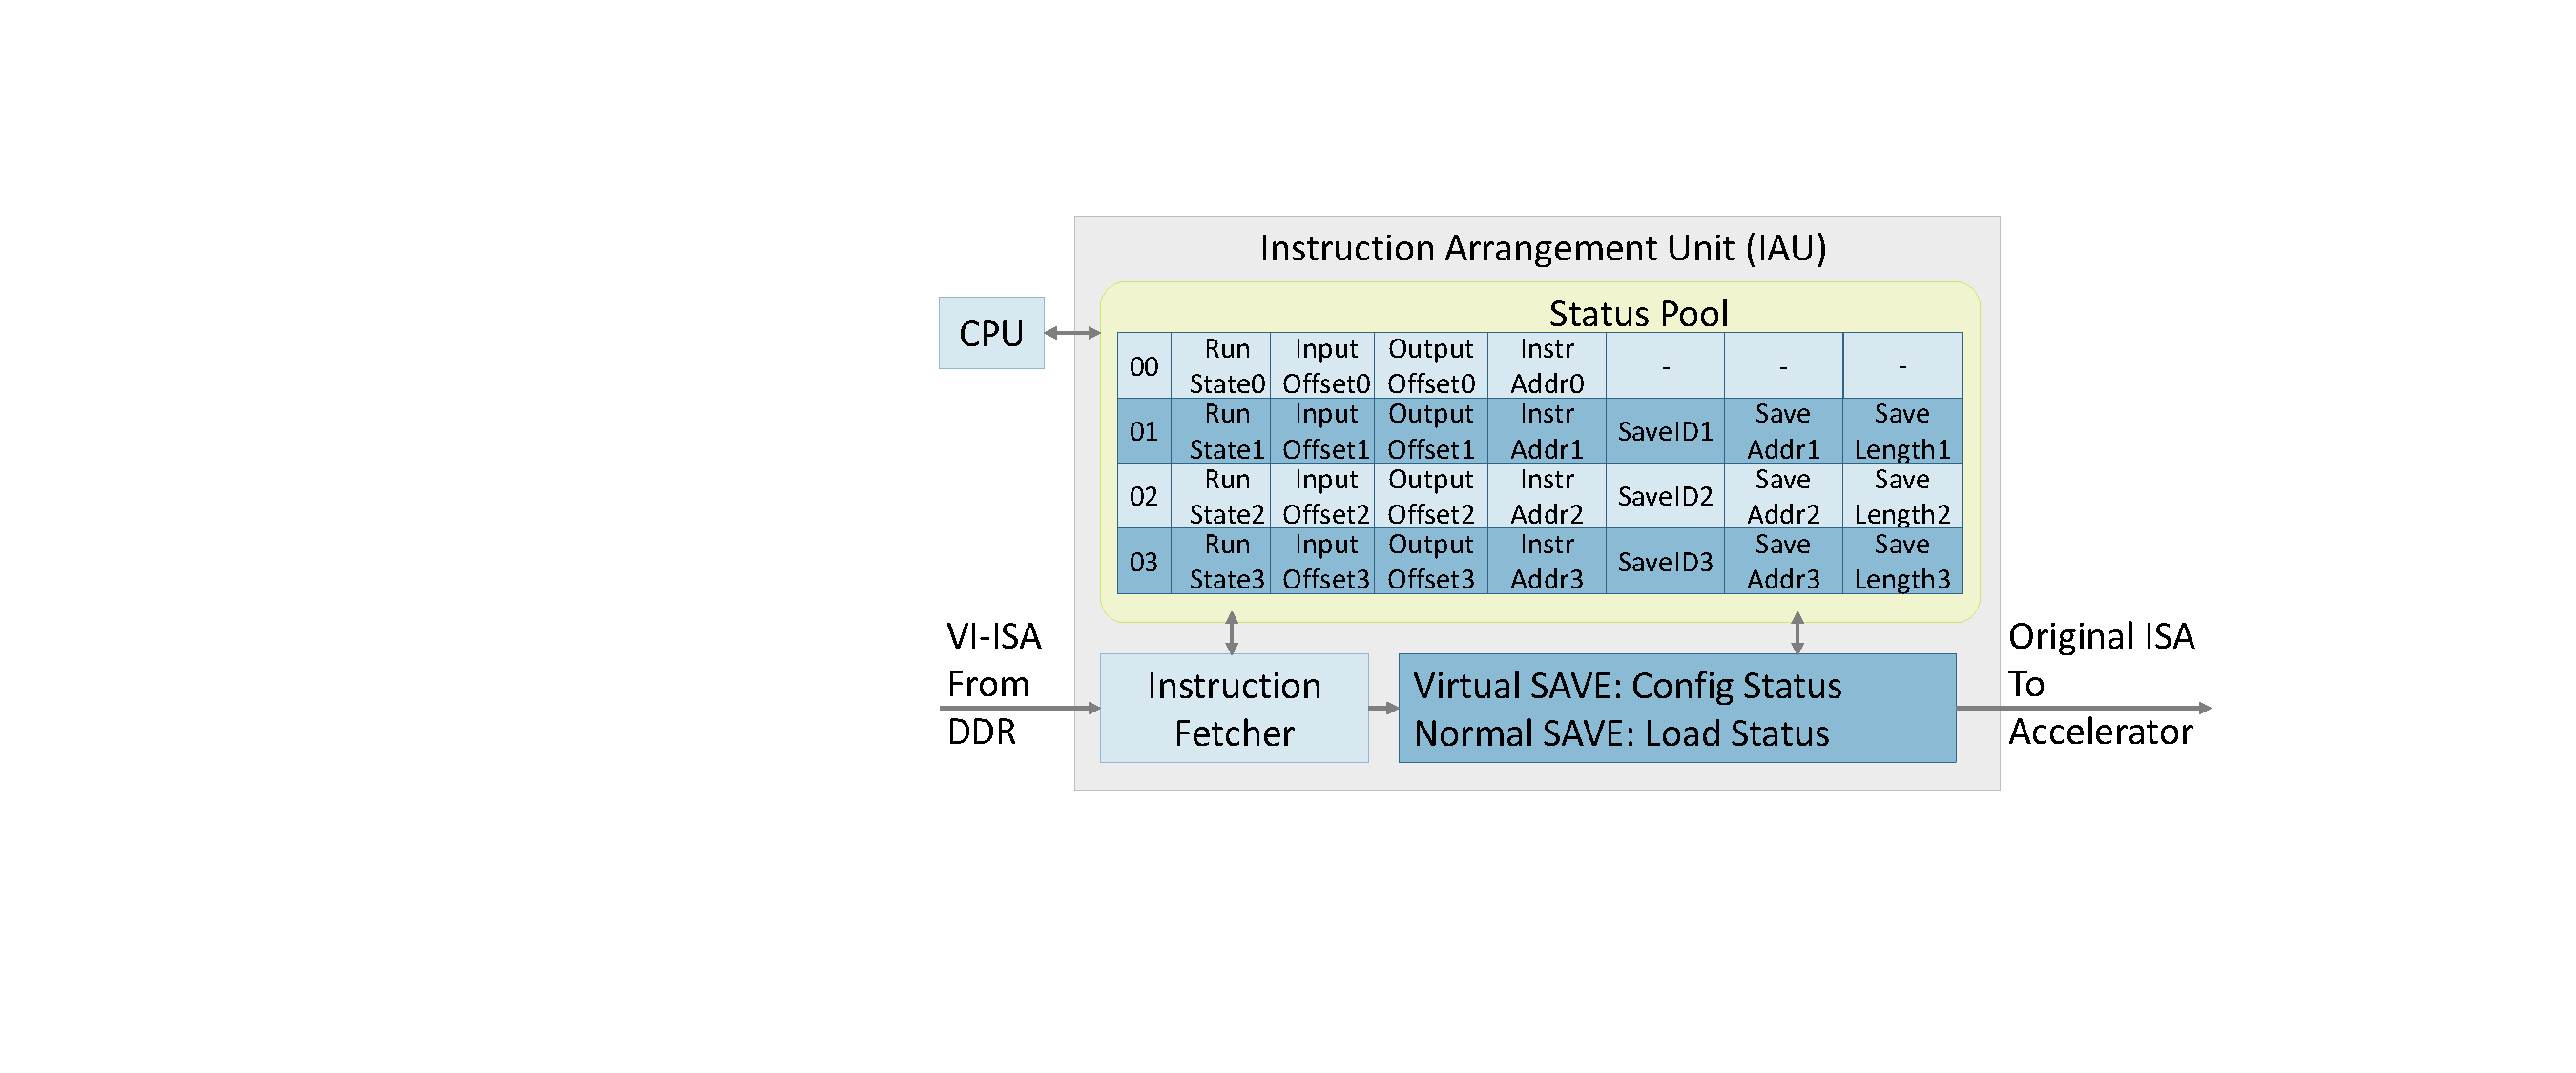
\includegraphics[width=0.9\linewidth]{fig/iau.pdf}
	\caption{Hardware architecture of IAU. 
	% The software on the CPU (PS side) communicates with IAU to access the CNN accelerator. IAU records the running state of each task. At runtime, IAU translates the input instruction sequence with virtual instructions to a normal sequence of instructions. IAU also modifies the normal SAVE instruction after interrupt occurs with the same SaveID, to avoid duplicate output data transfer. 
	}
	\label{fig:IAU}
\end{figure}

\begin{figure}[t]
	\centering
    % \vspace{-0.1cm} 
    % \setlength{\abovecaptionskip}{0cm} 
    % \setlength{\belowcaptionskip}{-0.05cm} 
	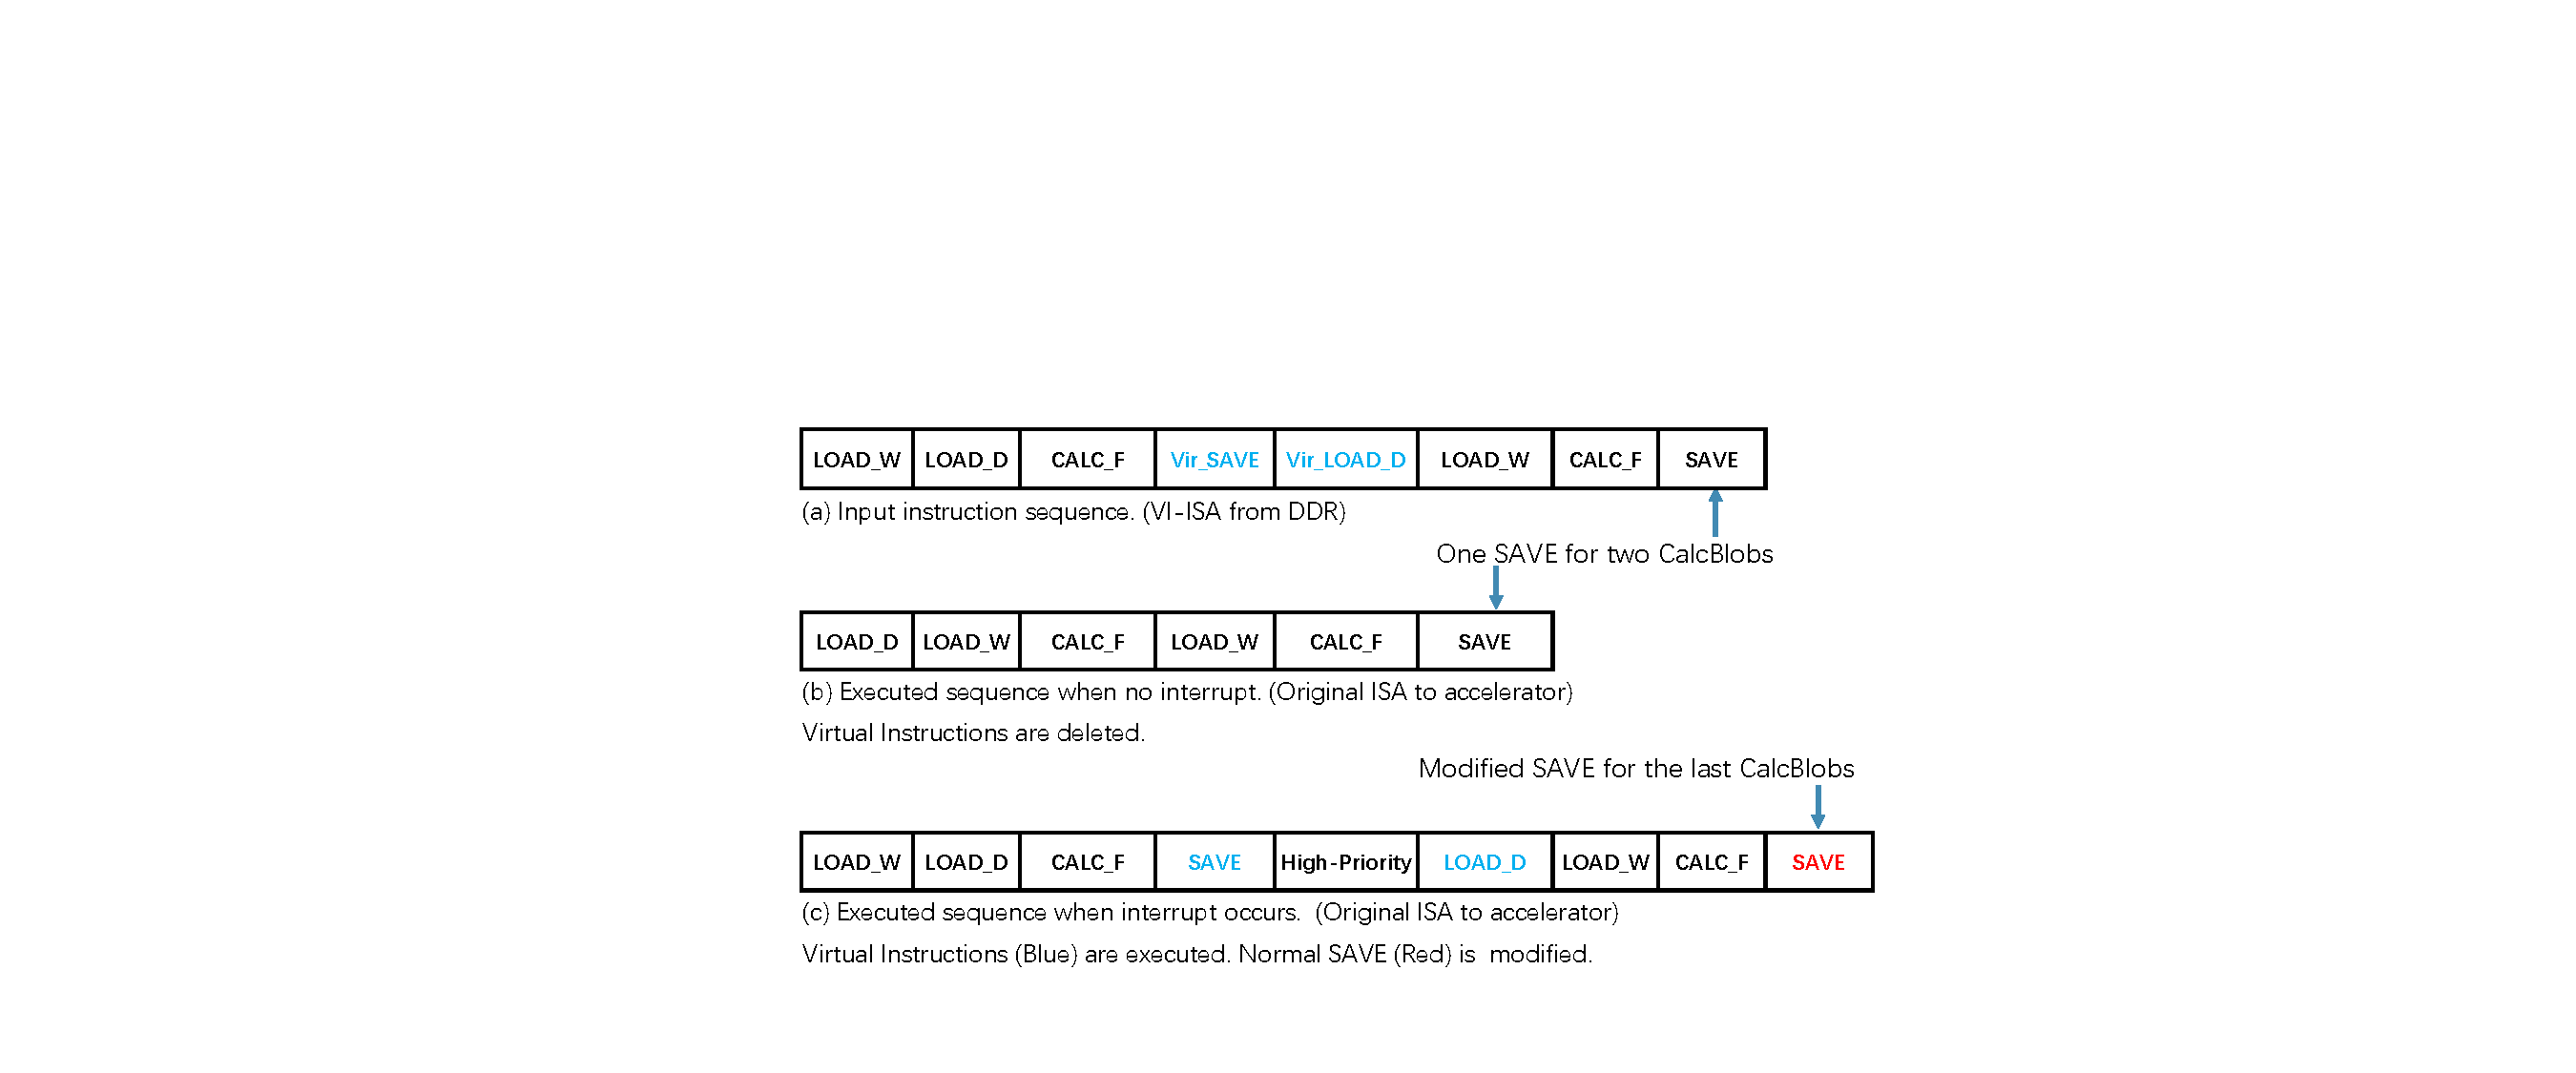
\includegraphics[width=0.9\linewidth]{fig/interexample.pdf}
	\caption{ A simple example of our proposed virtual-instruction-based interrupt. }
	\label{fig:interexample}
\end{figure}

\Cref{fig:interexample}(c) is the instruction sequence from DDR with VI-ISA. The instructions are generated for the scheduling shown in {fig:singlesave}. 
\Cref{fig:interexample}(d) is the original ISA instructions translated by the IAU without interrupt. 
When an interrupt occurs at the first CalcBlob, \Cref{fig:interexample}(e) illustrates the backup/recovery instructions (Blue) and the modified SAVE instruction (Red). 